\smallframetitle

\section{From 01/07/24 to 05/07/24}
\insertsectionframe

\subsection{New road detection method}
\insertsubsectionframe

\begin{frame}{Building city connection graph (1/4)}
    \begin{columns}
        \begin{column}{0.4\textwidth}
            \begin{block}{City detection}
                A clustering method (here DBScan) is used only on the base station detected as a city center by the 3NN method.
                Thus, these base stations are now separated in different cities.
            \end{block}
        \end{column}
        \begin{column}{0.6\textwidth}
            \begin{figure}
                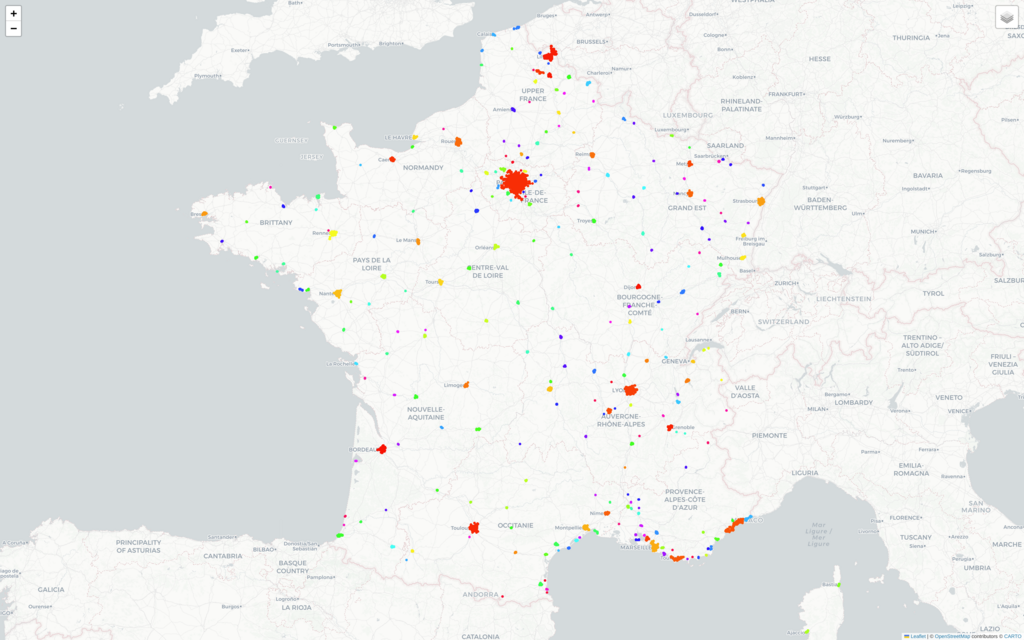
\includegraphics[width=0.5\paperwidth]{images/road_detection/city_clustering.png}
                \caption{city clustering}
            \end{figure}
        \end{column}
    \end{columns}        
\end{frame}

\begin{frame}{Building city connection graph (2/4)}
    \begin{columns}
        \begin{column}{0.4\textwidth}
            \begin{block}{Center computation}
                The center of each cluster is computed.
            \end{block}

            \begin{block}{city separation according to size}
                The cities that contain more than a certain number of stations are separated from the ones that contain less.
            \end{block}
        \end{column}
        \begin{column}{0.6\textwidth}
            \begin{figure}
                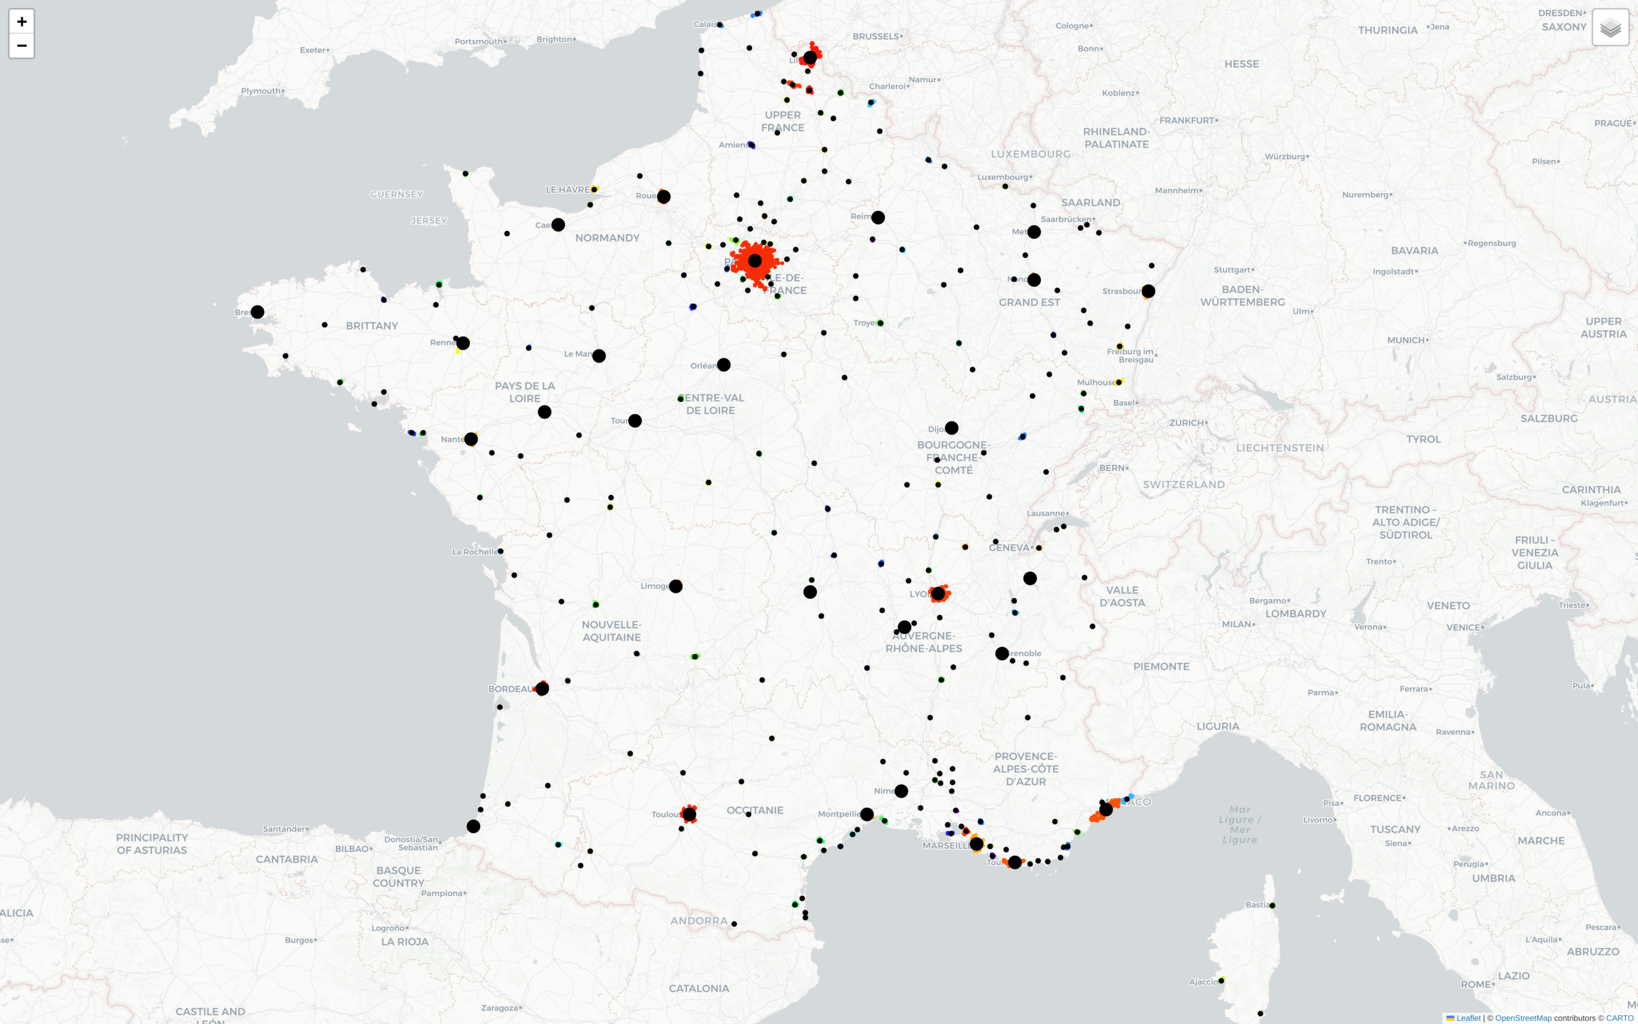
\includegraphics[width=0.5\paperwidth]{images/road_detection/city_clustering_with_centers.png}
                \caption{cities centers and size classification}
            \end{figure}
        \end{column}
    \end{columns}        
\end{frame}

\begin{frame}{Building city connection graph (3/4)}
    \begin{columns}
        \begin{column}{0.4\textwidth}
            \begin{block}{Delaunay triangulation}
                The Delaunay traingulation is then applied to the big cities to create a graph.
            \end{block}
        \end{column}
        \begin{column}{0.6\textwidth}
            \begin{figure}
                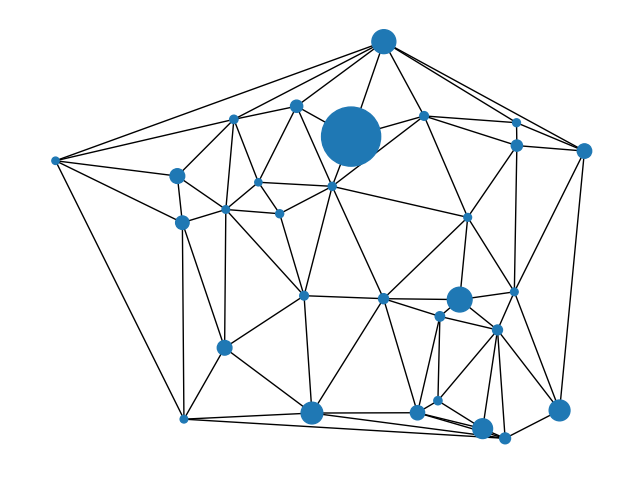
\includegraphics[height=0.3\paperheight]{images/road_detection/delaunay_big_cities_unfiltered.png}
                \caption{Big cities connection graph unfiltered}
            \end{figure}
        \end{column}
    \end{columns}        
\end{frame}

\begin{frame}{Building city connection graph (4/4)}
    \begin{block}{Graph filtration}
        The angle and distance criteria are then applied to filter the connections between the cities.
    \end{block}
    \begin{columns}
        \begin{column}{0.3\textwidth}
            \begin{figure}
                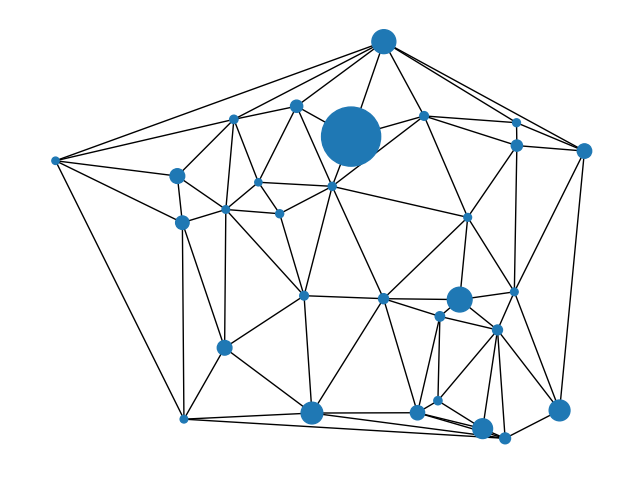
\includegraphics[width=0.2\paperwidth]{images/road_detection/delaunay_big_cities_unfiltered.png}
                \caption{Unfiltered}
            \end{figure}
        \end{column}
        \begin{column}{0.3\textwidth}
            \begin{figure}
                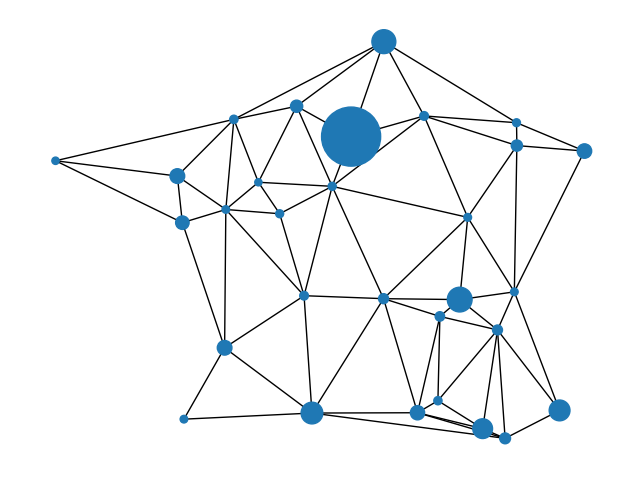
\includegraphics[width=0.2\paperwidth]{images/road_detection/delaunay_big_cities_distance_filtered.png}
                \caption{Distance filtered}
            \end{figure}
        \end{column}
        \begin{column}{0.3\textwidth}
            \begin{figure}
                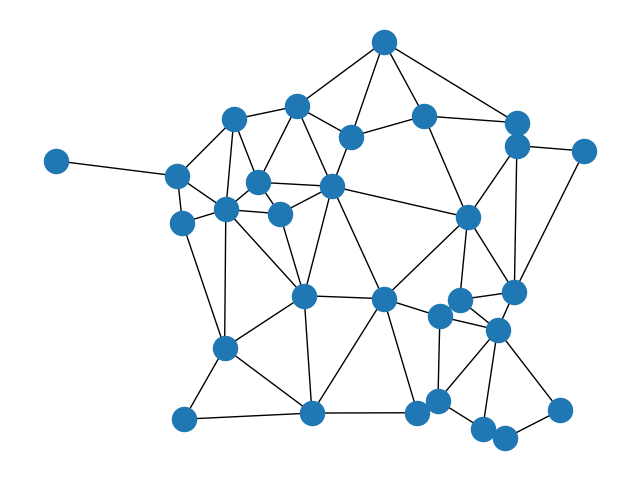
\includegraphics[width=0.2\paperwidth]{images/road_detection/delaunay_big_cities_distance_angle_filtered.png}
                \caption{Distance and angle filtered}
            \end{figure}
        \end{column}
    \end{columns}        
\end{frame}